\documentclass[a4paper,11pt]{article}
\input{/home/tof/Documents/Cozy/latex-include/preambule_lua.tex}
\newcommand{\showprof}{show them}  % comment this line if you don't want to see todo environment
\fancyhead[L]{Correction exercices arbre}
\newdate{madate}{10}{09}{2020}
%\fancyhead[R]{\displaydate{madate}} %\today
%\fancyhead[R]{Seconde - SNT}
%\fancyhead[R]{Première - NSI}
\fancyhead[R]{Terminale - NSI}
\fancyfoot[L]{~\\Christophe Viroulaud}
\AtEndDocument{\label{lastpage}}
\fancyfoot[C]{\textbf{Page \thepage/\pageref{lastpage}}}
\fancyfoot[R]{\includegraphics[width=2cm,align=t]{/home/tof/Documents/Cozy/latex-include/cc.png}}
\usepackage{tikz}

\begin{document}
\begin{Form}
\begin{exo}
\begin{enumerate}
\item \begin{itemize}
\item racine: A
\item 8 feuilles
\item taille: 16
\item profondeur: 3
\end{itemize}
\item \begin{itemize}
\item parcours en largeur: A B C D E F N G H I J K L O P M
\item parcours en profondeur: A B C F K L N D G O P H I M E J
\end{itemize}
\end{enumerate}
\end{exo}
\begin{exo}
\begin{itemize}
\item Windows: taille = 22; hauteur = 2
\item Linux: taille = 35; hauteur = 3
\end{itemize}
\end{exo}
\begin{exo}
\begin{enumerate}
\item liste
\begin{lstlisting}
dictionnaire = ['arbre', 'arbres', 'arbitre', 'arbitrent', 'arbitrer', 'arbitres', 'arbitrez', 'arbitrons', 'binaire', 'binaires', 'binette', 'binettes', 'bio', 'empile', 'empilent' 'empiler', 'empiles', 'empilez', 'empilons', 'exact', 'exacte', 'exactes', 'exacts']
\end{lstlisting}
23 éléments dans la liste et 22 tests pour trouver \emph{exactes}.
\item arbre
\begin{center}
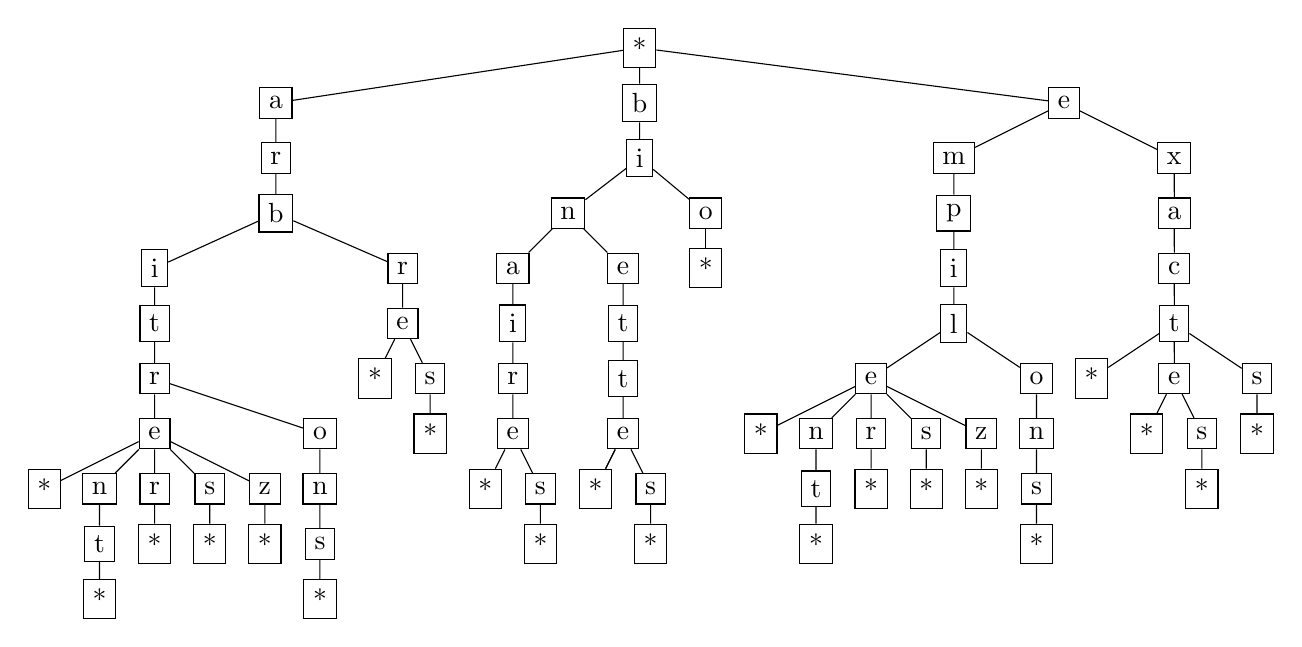
\begin{tikzpicture}[scale=0.7]
\node[draw] (0) at (-11,0) {*};
\node[draw] (1) at (-7,0) {*};
\node[draw] (3) at (-11,1) {t};
\node[draw] (4) at (-10,1) {*};
\node[draw] (5) at (-9,1) {*};
\node[draw] (6) at (-8,1) {*};
\node[draw] (7) at (-7,1) {s};
\node[draw] (8) at (-3,1) {*};
\node[draw] (9) at (-1,1) {*};
\node[draw] (10) at (2,1) {*};
\node[draw] (11) at (6,1) {*};
\node[draw] (12) at (-12,2) {*};
\node[draw] (13) at (-11,2) {n};
\node[draw] (14) at (-10,2) {r};
\node[draw] (15) at (-9,2) {s};
\node[draw] (16) at (-8,2) {z};
\node[draw] (17) at (-7,2) {n};
\node[draw] (18) at (-4,2) {*};
\node[draw] (19) at (-3,2) {s};
\node[draw] (20) at (-2,2) {*};
\node[draw] (21) at (-1,2) {s};
\node[draw] (22) at (2,2) {t};
\node[draw] (23) at (3,2) {*};
\node[draw] (24) at (4,2) {*};
\node[draw] (25) at (5,2) {*};
\node[draw] (26) at (6,2) {s};
\node[draw] (27) at (9,2) {*};
\node[draw] (28) at (-10,3) {e};
\node[draw] (29) at (-7,3) {o};
\node[draw] (30) at (-5,3) {*};
\node[draw] (31) at (-3.5,3) {e};
\node[draw] (32) at (-1.5,3) {e};
\node[draw] (33) at (1,3) {*};
\node[draw] (34) at (2,3) {n};
\node[draw] (35) at (3,3) {r};
\node[draw] (36) at (4,3) {s};
\node[draw] (37) at (5,3) {z};
\node[draw] (38) at (6,3) {n};
\node[draw] (39) at (8,3) {*};
\node[draw] (40) at (9,3) {s};
\node[draw] (41) at (10,3) {*};
\node[draw] (42) at (-10,4) {r};
\node[draw] (43) at (-6,4) {*};
\node[draw] (44) at (-5,4) {s};
\node[draw] (45) at (-3.5,4) {r};
\node[draw] (46) at (-1.5,4) {t};
\node[draw] (47) at (3,4) {e};
\node[draw] (48) at (6,4) {o};
\node[draw] (49) at (7,4) {*};
\node[draw] (50) at (8.5,4) {e};
\node[draw] (51) at (10,4) {s};
\node[draw] (52) at (-10,5) {t};
\node[draw] (53) at (-5.5,5) {e};
\node[draw] (54) at (-3.5,5) {i};
\node[draw] (55) at (-1.5,5) {t};
\node[draw] (56) at (4.5,5) {l};
\node[draw] (57) at (8.5,5) {t};
\node[draw] (58) at (-10,6) {i};
\node[draw] (59) at (-5.5,6) {r};
\node[draw] (60) at (-3.5,6) {a};
\node[draw] (61) at (-1.5,6) {e};
\node[draw] (62) at (0,6) {*};
\node[draw] (63) at (4.5,6) {i};
\node[draw] (64) at (8.5,6) {c};
\node[draw] (65) at (-7.8,7) {b};
\node[draw] (66) at (-2.5,7) {n};
\node[draw] (67) at (0,7) {o};
\node[draw] (68) at (4.5,7) {p};
\node[draw] (69) at (8.5,7) {a};
\node[draw] (70) at (-7.8,8) {r};
\node[draw] (71) at (-1.2,8) {i};
\node[draw] (72) at (4.5,8) {m};
\node[draw] (73) at (8.5,8) {x};
\node[draw] (74) at (-7.8,9) {a};
\node[draw] (75) at (-1.2,9) {b};
\node[draw] (76) at (6.5,9) {e};
\node[draw] (77) at (-1.2,10) {*};

\draw (0) -- (3);
\draw (1) -- (7);
\draw (3) -- (13);
\draw (4) -- (14);
\draw (5) -- (15);
\draw (6) -- (16);
\draw (7) -- (17);
\draw (8) -- (19);
\draw (9) -- (21);
\draw (10) -- (22);
\draw (11) -- (26);
\draw (12) -- (28);
\draw (13) -- (28);
\draw (14) -- (28);
\draw (15) -- (28);
\draw (16) -- (28);
\draw (17) -- (29);
\draw (18) -- (31);
\draw (19) -- (31);
\draw (20) -- (32);
\draw (20) -- (32);
\draw (21) -- (32);
\draw (22) -- (34);
\draw (23) -- (35);
\draw (24) -- (36);
\draw (25) -- (37);
\draw (26) -- (38);
\draw (27) -- (40);
\draw (28) -- (42);
\draw (30) -- (44);
\draw (31) -- (45);
\draw (32) -- (46);
\draw (33) -- (47);
\draw (34) -- (47);
\draw (35) -- (47);
\draw (36) -- (47);
\draw (37) -- (47);
\draw (38) -- (48);
\draw (39) -- (50);
\draw (40) -- (50);
\draw (41) -- (51);
\draw (42) -- (29);
\draw (42) -- (52);
\draw (43) -- (53);
\draw (44) -- (53);
\draw (45) -- (54);
\draw (46) -- (55);
\draw (47) -- (56);
\draw (48) -- (56);
\draw (49) -- (57);
\draw (50) -- (57);
\draw (51) -- (57);
\draw (52) -- (58);
\draw (53) -- (59);
\draw (54) -- (60);
\draw (55) -- (61);
\draw (56) -- (63);
\draw (57) -- (64);
\draw (58) -- (65);
\draw (59) -- (65);
\draw (60) -- (66);
\draw (61) -- (66);
\draw (62) -- (67);
\draw (63) -- (68);
\draw (64) -- (69);
\draw (65) -- (70);
\draw (66) -- (71);
\draw (67) -- (71);
\draw (68) -- (72);
\draw (69) -- (73);
\draw (70) -- (74);
\draw (71) -- (75);
\draw (72) -- (76);
\draw (73) -- (76);
\draw (74) -- (77);
\draw (75) -- (77);
\draw (76) -- (77);

\end{tikzpicture}
\captionof{figure}{Dictionnaire}
\label{dico}
\end{center}
8 tests pour trouver \emph{exactes} (en toute rigueur un peu plus).
\end{enumerate}
\end{exo}

\begin{exo}

\begin{enumerate}
\item Arbre (presque complet)
\begin{center}
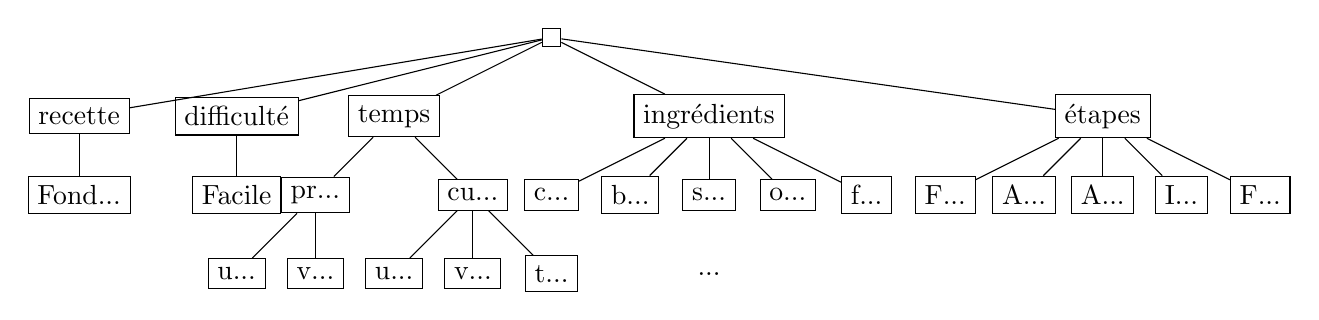
\begin{tikzpicture}
\node[draw] (A) at (0,0) {};
\node[draw] (B) at (-6,-1) {recette};
\node[draw] (C) at (-4,-1) {difficulté};
\node[draw] (D) at (-2,-1) {temps};
\node[draw] (E) at (2,-1) {ingrédients};
\node[draw] (F) at (7,-1) {étapes};
\node[draw] (N) at (-6,-2) {Fond...};
\node[draw] (G) at (-4,-2) {Facile};
\node[draw] (H) at (-3,-2) {pr...};
\node[draw] (I) at (-1,-2) {cu...};
\node[draw] (J) at (0,-2) {c...};
\node[draw] (K) at (1,-2) {b...};
\node[draw] (L) at (2,-2) {s...};
\node[draw] (M) at (3,-2) {o...};
\node[draw] (O) at (4,-2) {f...};
\node[draw] (P) at (5,-2) {F...};
\node[draw] (Q) at (6,-2) {A...};
\node[draw] (R) at (7,-2) {A...};
\node[draw] (S) at (8,-2) {I...};
\node[draw] (T) at (9,-2) {F...};
\node[draw] (U) at (-4,-3) {u...};
\node[draw] (V) at (-3,-3) {v...};
\node[draw] (W) at (-2,-3) {u...};
\node[draw] (X) at (-1,-3) {v...};
\node[draw] (Y) at (0,-3) {t...};
\node (Z) at (2,-3) {...};

\draw (A) -- (B);
\draw (A) -- (C);
\draw (A) -- (D);
\draw (A) -- (E);
\draw (A) -- (F);
\draw (B) -- (N);
\draw (C) -- (G);
\draw (D) -- (H);
\draw (D) -- (I);
\draw (E) -- (J);
\draw (E) -- (K);
\draw (E) -- (L);
\draw (E) -- (M);
\draw (E) -- (O);
\draw (F) -- (P);
\draw (F) -- (R);
\draw (F) -- (S);
\draw (F) -- (T);
\draw (F) -- (Q);
\draw (H) -- (U);
\draw (H) -- (V);
\draw (I) -- (W);
\draw (I) -- (X);
\draw (I) -- (Y);

\end{tikzpicture}
\captionof{figure}{Recette du fondant au chocolat}
\label{arbre}
\end{center}
\item Ouvrir le fichier \emph{recette.py}. L'arbre a été construit avec la classe \emph{Noeud}.
\item BFS
\lstinputlisting[firstline=18,lastline=28]{"scripts/recette-corrige.py"}
\item affichage
\lstinputlisting[firstline=30,lastline=37]{"scripts/recette-corrige.py"}
\end{enumerate}
\end{exo}


\end{Form}
\end{document}